\chapter{Асимметричные криптосистемы}\label{chapter-public-key}
\selectlanguage{russian}

\emph{Асимметричной криптосистемой} или же \emph{криптосистемой с открытым ключом} (\langen{public-key cryptosystem, PKC}) называется криптографическое преобразование, использующее два ключа -- открытый и закрытый. Пара из \emph{закрытого}\index{ключ!закрытый} (\langen{private key, secret key, SK})\footnote{В контексте криптосистем с открытым ключом можно ещё встретить использование термина <<секретный ключ>>. Мы не рекомендуем использовать данный термин, чтобы не путать с секретным ключом\index{ключ!секретный}, используемым в симметричных криптосистемах.} и \emph{открытого}\index{ключ!открытый} (\langen{public key, PK}) ключей создаётся пользователем, который свой закрытый ключ держит в секрете, а открытый ключ делает общедоступным для всех пользователей. Криптографическое преобразование в одну сторону (шифрование) можно выполнить, зная только открытый ключ, а в другую (расшифрование) -- зная только закрытый ключ. Во многих криптосистемах из открытого ключа теоретически можно вычислить закрытый ключ, однако это является сложной вычислительной задачей.

Если прямое преобразование выполняется открытым ключом, а обратное -- закрытым, то криптосистема называется \emph{схемой шифрования с открытым ключом}. Все пользователи, зная открытый ключ получателя, могут зашифровать для него сообщение, которое может расшифровать только владелец закрытого ключа.

Если прямое преобразование выполняется закрытым ключом, а обратное -- открытым, то криптосистема называется \emph{схемой электронной подписи (ЭП)}. Владелец закрытого ключа может \emph{подписать} сообщение, а все пользователи, зная открытый ключ, могут проверить, что подпись была создана только владельцем закрытого ключа и никем другим.

Криптосистемы с открытым ключом снижают требования к каналам связи, необходимые для передачи данных. В симметричных криптосистемах перед началом связи (перед шифрованием сообщения и его передачей) требуется передать или согласовать секретный ключ шифрования по защищённому каналу связи. Злоумышленник не должен иметь возможности ни прослушать данный канал связи, ни подменить передаваемую информацию (ключ). Для надёжной работы криптосистем с открытым ключом необходимо, чтобы злоумышленник не имел возможности подменить открытый ключ легального пользователя. Другими словами, криптосистема с открытым ключом, в случае использования открытых и незащищённых каналов связи, устойчива к действиям пассивного криптоаналитика\index{криптоаналитик!пассивный}, но всё ещё должна предпринимать меры по защите от активного криптоаналитика\index{криптоаналитик!активный}.

Для предотвращения атак <<человек посередине>> (\langen{man-in-the-middle attack})\index{атака!<<человек посередине>>} с активным криптоаналитиком\index{криптоаналитик!активный}, который бы подменял открытый ключ получателя во время его передачи будущему отправителю сообщений, используют \emph{сертификаты открытых ключей}\index{сертификат открытого ключа}. Сертификат представляет собой информацию о соответствии открытого ключа и его владельца, подписанную электронной подписью третьего лица. В корпоративных информационных системах организация может обойтись одним лицом, подписывающим сертификаты. В этом случае его называют \emph{доверенным центром сертификации} или \emph{удостоверяющим центром}. В глобальной сети Интернет для защиты распространения программного обеспечения (например, защиты от подделок в ПО) и проверок сертификатов в протоколах на базе SSL/TLS\index{протокол!SSL/TLS} используется иерархия удостоверяющих центров, рассмотренная в разделе~\ref{section-CAs}. При обмене личными сообщениями и при распространении программного обеспечения с открытым кодом вместо жёсткой иерархии может использоваться \emph{сеть доверия}\index{сеть доверия}. В сети доверия каждый участник может подписать сертификат любого другого участника. Предполагается, что подписывающий знает лично владельца сертификата и удостоверился в соответствии сертификата владельцу при личной встрече.

Криптосистемы с открытым ключом построены на основе односторонних (однонаправленных) функций с потайным входом. Под \emph{односторонней} функцией понимают такое отображение, которое подразумевает \emph{вычислительную} невозможность нахождения обратного отображения: вычисление значения функции $y = f(x)$ при заданном аргументе $x$ является лёгкой задачей, вычисление аргумента $x$ при заданном значении функции $y$ -- трудной задачей.

Односторонняя функция $y = f(x,K)$ с \emph{потайным входом}\index{функция!с потайным входом} $K$ определяется как функция, которая легко вычисляется при заданном $x$ и аргумент $x$ которой можно легко вычислить из $y$, если известен <<секретный>> параметр $K$, и вычислить невозможно, если параметр $K$ неизвестен.

Примером подобной функции является возведение в степень по модулю составного числа $n$:
	\[ c = f \left( m \right) = m ^ e \mod n.\]

Для того чтобы быстро вычислить обратную функцию
	\[ m = f^{-1} \left( c \right) = \sqrt[e]{c} \mod n, \]
её можно представить в виде
	\[ m = c^{d} \mod n,\]
где
	\[ d = e^{-1} \mod \varphi \left( n \right). \]

В последнем выражении $\varphi \left( n \right)$ -- это функция Эйлера\index{функция!Эйлера}. В качестве <<потайной дверцы>> или секрета можно рассматривать или непосредственно само число $d$, или значение $\varphi \left( n \right)$. Последнее можно быстро найти только в том случае, если известно разложение числа $n$ на простые сомножители. Именно эта функция с потайной дверцей лежит в основе криптосистемы RSA\index{криптосистема!RSA}.

Необходимые математические основы модульной арифметики, групп, полей и простых чисел приведены в приложении~\ref{chap:discrete-math}.

\section{Криптосистема RSA}\index{криптосистема!RSA|(}
\selectlanguage{russian}

\subsection{Шифрование}\index{шифр!RSA|(}

В 1978 г. Рональд Рив\'{е}ст, Ади Шамир и Леонард Адлеман (\langen{Ronald Linn Rivest, Adi Shamir, Leonard Max Adleman}, \cite{RSA:1978}) предложили алгоритм, обладающий рядом интересных для криптографии свойств. На его основе была построена первая система шифрования с открытым ключом, получившая название по первым буквам фамилий авторов -- система RSA.

Рассмотрим принцип построения криптосистемы шифрования RSA с открытым ключом.

\begin{enumerate}
    \item \textbf{Создание пары из закрытого и открытого ключей}
        \begin{enumerate}
            \item Случайно выбрать большие простые\index{число!простое} различные числа $p$ и $q$, для которых $\log_2 p \simeq \log_2 q > 1024$ бита\footnote{Случайный выбор больших простых чисел не является простой задачей. См. раздел~\ref{section-pseudo-primes-generation} в приложении.}.
            \item Вычислить произведение $n = pq$.
            \item Вычислить функцию Эйлера\index{функция!Эйлера}\footnote{См. раздел~\ref{section-group-multiplicative} в приложении.} $\varphi(n) = (p-1)(q-1)$.
            \item Выбрать случайное целое число $e \in [3, \varphi(n)-1]$, взаимно простое с $\varphi(n)$: $~ \gcd(e, \varphi(n)) = 1$.
            \item Вычислить число $d$ такое, что $d \cdot e = 1 \mod \varphi(n)$.
            \item Закрытым ключом будем называть пару чисел $n$ и $d$, открытым ключом\footnote{Некоторые авторы считают некорректным включать число $n$ в состав закрытого ключа, так как оно уже входит в открытый. Авторы настоящего пособия включают число $n$ в состав закрытого ключа, что в результате позволяет в дальнейшем использовать для расшифрования и создания электронной подписи данные \emph{только} из закрытого ключа, не прибегая к <<помощи>> данных из открытого ключа.} -- пару чисел $n$ и $e$.
        \end{enumerate}

    \item \textbf{Шифрование с использованием открытого ключа.}
        \begin{enumerate}
            \item Сообщение представляют целым числом $m \in [1, n-1]$.
            \item Шифртекст вычисляется как
                \[ c = m^e \mod n. \]
                Шифртекст -- также целое число из диапазона $[1, n-1]$.
        \end{enumerate}
    \item \textbf{Расшифрование с использованием закрытого ключа.}

        Владелец закрытого ключа вычисляет
                \[ m = c^d \mod n. \]
\end{enumerate}

Покажем корректность схемы шифрования RSA. В результате расшифрования шифртекста $c$ (полученного путём шифрования открытого текста $m$) легальный пользователь имеет:
\[\begin{array}{ll}
    c^{d} & = m^{ed} \mod p = \\
          & = m^{ 1 + \alpha_1 \cdot \varphi(n)} \mod p = \\
          & = m^{ 1 + \alpha_1 \cdot ( p - 1 ) ( q - 1 )} \mod p = \\
          & = m^{ 1 + \alpha_2 \cdot ( p - 1 )} \mod p = \\
          & = m \cdot m^{\alpha_2 \cdot ( p - 1 )} \mod p. \\
\end{array}\]

Если $m$ и $p$ являются взаимно простыми, то из малой теоремы Ферма\index{теорема!Ферма малая} следует, что:
	\[m^{\left( p - 1 \right)} = 1 \mod p,\]
\[\begin{array}{ll}
	c^{d} & = m \cdot m^{\alpha_2 \cdot \left( p - 1 \right)} = \\
	      & = m \cdot \left( m^{\left(p - 1\right)} \right)^{\alpha_2} = \\
	      & = m \cdot 1^{\alpha_2} = \\
	      & = m \mod p.
\end{array}\]

Если же $m$ и $p$ не являются взаимно простыми, то есть $p$ является делителем $m$ (помним, что $p$ -- простое число), то $m = 0 \mod p$ и $c^{d} = 0 \mod p$.

В результате, для любых $m$ верно, что $c^{d} = m \mod p$. Аналогично доказывается, что $c^{d} = m \mod q$. Из китайской теоремы об остатках\index{теорема!китайская об остатках} (см. раздел~\ref{section-chinese-remainder-theorem} в приложении) следует:
\[\begin{cases}
	n = p \cdot q, \\
	c^{d} = m \mod p, \\
	c^{d} = m \mod q.
\end{cases} \Rightarrow\quad c^{d} = m \mod n.\]

\example Создание ключей, шифрование и расшифрование в криптосистеме RSA.

\begin{enumerate}
    \item Генерирование параметров.
        \begin{enumerate}
            \item Выберем числа $p=13, q=11, n = 143$.
            \item Вычислим $\varphi(n) = (p-1)(q-1) = 12 \cdot 10 = 120$.
            \item Выберем $e=23: ~ \gcd(e, \varphi(n))=1, ~ e \in [3, 119]$.
            \item Найдём $d = e^{-1} \bmod \varphi(n) = 23^{-1} \bmod 120 = 47$.
            \item Открытый и закрытый ключи:
                \[ \PK = (e:23, n:143), ~ \SK = (d:47, n:143). \]
        \end{enumerate}
    \item Шифрование.
        \begin{enumerate}
            \item Пусть сообщение $m = 22 \in [1, n-1]$.
            \item Вычислим шифртекст:
                \[ c = m^e \bmod n = 22^{23} \bmod 143 = 55 \bmod 143. \]
        \end{enumerate}
    \item Расшифрование.
        \begin{enumerate}
            \item Полученный шифртекст $c = 55$.
            \item Вычислим открытый текст:
                \[ m = c^d \bmod n = 55^{47} \bmod 143 = 22 \bmod 143. \]
        \end{enumerate}
\end{enumerate}
\exampleend

\index{шифр!RSA|)}

\subsection{Электронная подпись}\index{электронная подпись!RSA|(}

Предположим, что пользователь $A$ не шифрует свои сообщения, но хочет посылать их в виде открытых текстов с подписью. Для этого надо создать электронную подпись (ЭП). Это можно сделать, используя систему RSA. При этом должны быть выполнены следующие требования:
\begin{itemize}
    \item вычисление подписи от сообщения является вычислительно лёгкой задачей;
    \item фальсификация подписи при неизвестном закрытом ключе -- вычислительно трудная задача;
    \item подпись должна быть проверяемой открытым ключом.
\end{itemize}

Создание параметров ЭП RSA производится так же, как и для схемы шифрования RSA. Пусть $A$ имеет закрытый ключ $\SK = (n, d)$, а получатель (проверяющий) $B$ -- открытый ключ $\PK = (e,n)$ пользователя $A$.

\begin{enumerate}
    \item $A$ вычисляет подпись сообщения $m \in [1,n-1]$ как
        \[ s = m^{d} \mod n \]
        на своём закрытом ключе $\SK$.
    \item $A$ посылает $B$ сообщение в виде $(m, s)$, где $m$ -- открытый текст, $s$ -- подпись.
    \item $B$ принимает сообщение $(m, s)$, возводит $s$ в степень $e$ по модулю $n$ ($e, n$ -- часть открытого ключа). В результате вычислений $B$ получает открытый текст:
        \[ s^{e} \mod n = \left( m^{d} \mod n \right)^{e} \mod n = m. \]
    \item $B$ cравнивает полученное значение с первой частью сообщения. При полном совпадении подпись принимается.
\end{enumerate}
Недостаток данной системы создания ЭП состоит в том, что подпись $m^{d} \mod n$ имеет большую длину, равную длине открытого сообщения $m$.

Для уменьшения длины подписи применяется другой вариант процедуры: вместо сообщения $m$ отправитель подписывает $h(m)$, где $h(x)$ -- известная криптографическая хэш-функция. Модифицированная процедура состоит в следующем.

\begin{enumerate}
    \item $A$ посылает $B$ сообщение в виде $(m, s)$, где $m$ -- открытый текст,
        \[ s = h(m)^d \mod n \]
        -- подпись.
    \item $B$ принимает сообщение $(m, s)$, вычисляет хэш $h(m)$ и возводит подпись в степень:
        \[ h_1 = s^e \mod n. \]
    \item $B$ сравнивает значения $h(m)$ и $h_1$. При равенстве
        \[ h(m) = h_1 \]
        подпись считается подлинной, при неравенстве -- фальсифицированной.
\end{enumerate}


\example Создание и проверка электронной подписи в криптосистеме RSA.

\begin{enumerate}
    \item Генерирование параметров.
        \begin{enumerate}
            \item Выберем $p=13, q=17, n = 221$.
            \item Вычислим $\varphi(n) = (p-1)(q-1) = 12 \cdot 16 = 192$.
            \item Выберем $e=25: ~ \gcd(e = 25, \varphi(n) = 192) = 1, \\
                e \in [3, \varphi(n) - 1 = 191]$.
            \item Найдём $d = e^{-1} \mod \varphi(n) = 25^{-1} \mod 192 = 169$.
            \item Открытый и закрытый ключи:
                \[ \PK = (e:25, n:221), ~ \SK = (d:169, n:221). \]
        \end{enumerate}
    \item Подписание.
        \begin{enumerate}
            \item Пусть хэш сообщения $h(m) = 12 \in [1, n-1]$.
            \item Вычислим ЭП:
                \[ s = h^d = 12^{169} = 90 \mod 221. \]
        \end{enumerate}
    \item Проверка подписи.
        \begin{enumerate}
            \item Пусть хэш полученного сообщения $h(m) = 12$, полученная подпись $s = 90$.
            \item Выполним проверку:
                \[ h_1 = s^e = 90^{25} = 12 \mod 221, ~~ h_1 = h. \]
                Подпись верна.
        \end{enumerate}
\end{enumerate}

\index{электронная подпись!RSA|)}

\subsection{Семантическая безопасность шифров}

\emph{Семантически безопасной}\index{криптосистема!семантически-безопасная} называется криптосистема, для которой вычислительно невозможно извлечь любую информацию из шифртекстов, кроме длины шифртекста. Алгоритм RSA не является семантически безопасным. Одинаковые сообщения шифруются одинаково, и, следовательно, применима атака на различение сообщений.

Кроме того, сообщения длиной менее $\frac{k}{3}$ бит, зашифрованные на малой экспоненте $e=3$, \emph{дешифруются} нелегальным пользователем извлечением обычного кубического корня.

В приложениях RSA используется только в сочетании с рандомизацией\index{рандомизация шифрования}. В стандарте PKCS\#1 RSA Laboratories описана схема рандомизации перед шифрованием OAEP-RSA (\langen{Optimal Asymmetric Encryption Padding}). Примерная схема:
\begin{enumerate}
    \item Выбирается случайное $r$.
    \item Для открытого текста $m$ вычисляется
        \[ x = m \oplus H_1(r), ~ y = r \oplus H_2(x), \]
        где $H_1$ и $H_2$ -- криптографические хэш-функции.
    \item Сообщение $M = x ~\|~ y$ далее шифруется RSA.
\end{enumerate}

Восстановление $m$ из $M$ при расшифровании:
    \[ r = y \oplus H_2(x), ~ m = x \oplus H_1(r). \]

В модификации OAEP+ $x$ вычисляется как
    \[ x = \left( m \oplus H_1 \left( r \right) \right) \Vert \left. H_3 \left( m \Vert r \right) \right. .\]

В описанной выше схеме ЭП под $m$ понимается хэш открытого текста, вместо шифрования выполняется подписание, вместо расшифрования -- проверка подписи.


\subsection{Выбор параметров и оптимизация}

\subsubsection{Выбор экспоненты $e$}

В случайно выбранной экспоненте $e$ c битовой длиной $k = \lceil \log_2 e \rceil$ одна половина битов в среднем равна 0, другая -- 1. При возведении в степень $m^e \mod n$ по методу <<возводи в квадрат и перемножай>> получится $k-1$ возведений в квадрат и в среднем
 $\frac{1}{2}(k-1)$ умножений.

Если выбрать $e$, содержащую малое число единиц в двоичной записи, то число умножений уменьшится до числа единиц в $e$.

Часто экспонента $e$ выбирается \emph{малым} \emph{простым} числом и/или содержащим малое число единиц в битовой записи для ускорения шифрования или проверки подписи, например:
\[
    \begin{array}{l}
        3 = [11]_2, \\
        17 = 2^4+1 = [10001]_2, \\
        257 = 2^8+1 = [100000001]_2, \\
        65537 = 2^{16}+1 = [10000000000000001]_2.
    \end{array}
\]

%Время шифрования или проверки подписи для малых экспонент становится $O(k^2)$ вместо $O(k^3)$, то есть в сотни раз быстрее для 1000-битовых чисел.


\subsubsection{Ускорение~шифрования по~китайской~теореме об~остатках}

Возводя $m$ в степень $e$ отдельно по $\Mod p$ и $\Mod q$ и применяя китайскую теорему об остатках\index{теорема!китайская об остатках} (\langen{Chinese remainder theorem, CRT}), можно быстрее выполнить шифрование.

Однако ускорение шифрования в криптосистеме RSA через CRT может породить уязвимости в отдельных реализациях, например в реализациях для смарт-карт.

\example
Пусть $c = m^e \mod n$ передаётся на расшифрование на смарт-карту, где вычисляется
\[ \begin{array}{c}
    m_p = c^d \mod p, \\
    m_q = c^d \mod q, \\
    m = m_p q (q^{-1} \bmod p) + m_q p (p^{-1} \bmod q) \mod n. \\
\end{array} \]
Криптоаналитик внешним воздействием может вызвать сбой во время вычисления $m_p$ (или $m_q$), в результате получится $m_p'$ и $m'$ вместо $m$. Зная $m_p'$ и $m'$, криптоаналитик находит разложение числа $n$ на множители $p,q$:
    \[ \gcd(m' - m, ~ n) = \gcd( (m_p' - m) q (q^{-1} \bmod p), ~ pq) = q. \]
\exampleend


\subsubsection{Длина ключей}

В 2005 году было разложено 663-битовое число вида RSA. Время разложения в эквиваленте составило 75 лет вычислений одного ПК. Самые быстрые алгоритмы факторизации -- субэкспоненциальные\index{задача!факторизации}. Минимальная рекомендуемая длина модуля $n$ = 1024 бита, но лучше использовать 2048 или 4096 бит.

В июле 2012 года NIST опубликовала отчёт~\cite{NIST:SP800:57}, который включал в себя таблицу сравнения надёжности ключей разных длин для криптосистем, относящихся к разным классам. Таблица была составлена согласно как известным на тот момент атакам на классы криптосистем, так и на конкретные шифры (см. таблицу~\ref{table:aesrsakeycompare}).

\begin{table}[h]
\centering
\begin{tabular}{|C{0.2\linewidth}|C{0.2\linewidth}|C{0.2\linewidth}|C{0.2\linewidth}|}
\hline
бит безопасности & пример симметричного шифра & $\log_2 n$ для RSA\tablefootnote{Сравнимая по предоставляемой безопасности битовая длина произведения $n$ простых чисел $p$ и $q$ для криптосистем, основанных на сложности задачи разложения числа $n$ на простые множители $p$ и $q$, в том числе RSA.} & $\log_2 \| \group{G} \|$ для эллиптических кривых\tablefootnote{Сравнимая по предоставляемой безопасности битовая длина количества элементов $\|\group{G}\|$ в выбранной циклической подгруппе $\group{G}$ группы точек $\group{E}$ эллиптической кривой для криптосистем, основанных на сложности дискретного логарифма в группах точек эллиптических кривых над конечными полями (см.~\ref{section-elliptic-curve-cryptosystems}).} \\
\hline
80	& 	2TDEA	&	1024	&	160--223	\\
112	& 	3TDEA	&	2048	&	224--255	\\
128	& 	AES-128	&	3072	&	256--383	\\
192	& 	AES-192	&	7680	&	384--511	\\
256	& 	AES-256	&	15360	&	512+	\\
\hline
\end{tabular}
\caption{Сравнимые длины ключей блочных симметричных шифров и ключевых параметров асимметричных шифров~\cite{NIST:SP800:57}}\label{table:aesrsakeycompare}
\end{table}

В приложении~\ref{section-modular-arithmetic} показано, что битовая сложность (количество битовых операций) вычисления произвольной степени $a^b \mod n$ является кубической $O(k^3)$, а возведения в квадрат $a^2 \mod n$ и умножения $a b \mod n$ -- квадратичной $O(k^2)$, где $k$ -- битовая длина чисел $a,b,n$.

%Увеличение длины модуля $n$ в 2 раза увеличивает время возведения в степень в $2^3$ раз для большой экспоненты $e$, а для маленькой экспоненты -- в $2^2$ раза.

\index{криптосистема!RSA|)}


\subsection{Протокол Эль-Гамаля}\index{протокол!Эль-Гамаля|(}
\selectlanguage{russian}

\begin{figure}[thb]
	\centering
	\begin{sequencediagram}
		\newinst{Alice}{Alice}
		\newinst[2.5]{Bob}{Bob}

		\mess{Alice}{$ g^x \bmod p $}{Bob}
	\end{sequencediagram}
	\caption{Диаграмма последовательности взаимодействия участников в протоколе Эль-Гамаля\label{fig:key_distribution-el-gamal}}
\end{figure}

Протокол Эль-Гамаля (рис.~\ref{fig:key_distribution-el-gamal}, \cite{ElGamal:1984, ElGamal:1985}) за счёт предварительного распространения открытого ключа одной из сторон обеспечивает аутентификацию ключа для этой стороны. Можно гарантировать, что только владелец соответствующего закрытого ключа сможет вычислить сеансовый ключ. Однако подтверждение факта получение ключа (выполнение целей G1 и G8) не является частью протокола.

\begin{protocol}
    \item[(0)] Алиса и Боб выбирают общие параметры $p$ и $g$, где $p$ -- большое простое число, а $g$ -- примитивный элемент поля $\Z_p^*$.
    \item[{}] Боб создаёт пару из закрытого и открытого ключей $b$ и $K_B$:
        \[\begin{array}{l}
            b: 2 \leq b \leq p - 1, \\
            K_B = g^b \bmod p.
        \end{array}\]
    \item[{}] Открытый ключ $K_B$ находится в общем открытом доступе для всех сторон. Криптоаналитик не может подменить его -- подмена будет заметна.
    \item[(1)] Алиса выбирает секрет $x$ и вычисляет сеансовый ключ $K$
        \[ K = K_B^{x} = g^{bx} \bmod p. \]
        \[ Alice \to \left\{ g^x \bmod p \right\} \to Bob\]
    \item[(2)] Боб вычисляет сеансовый ключ
        \[ K = (g^x)^{b} = g^{bx} \bmod p. \]
\end{protocol}

Протокол не обеспечивает гарантию выбора нового сессионного ключа в каждом сеансе протокола (G10), а использование <<мастер>>-ключа $K_B$ для передачи сеансового ключа позволяет злоумышленнику вычислить все сессионные ключи из прошлых сеансов при компрометации закрытого ключа $b$ (цель G9).

\index{протокол!Эль-Гамаля|)}

\section{Эллиптические кривые}\label{section-elliptic-curve-cryptosystems}
\selectlanguage{russian}

Существуют аналоги криптосистемы Эль-Гамаля, в которых вместо проблемы дискретного логарифма в мультипликативных полях используется проблема дискретного логарифма в группах точек эллиптических кривых над конечными полями (обычно $GF(p)$ либо $GF(2^n)$). Математическое описание данных полей приведено в разделе~\ref{section-math-ec-groups}. Нас же интересует следующий факт: для группы точек эллиптической кривой над конечным полем $\group{E}$ существует быстро выполнимая операция -- умножение целого числа $x$ на точку $A$ (суммирование точки самой с собой целое число раз):
\[ \begin{array}{l}
	x \in \group{Z}, \\
	A, B \in \group{E}, \\
	B = x \times A. \\
\end{array} \]

И получение исходной точки $A$ при известных $B$ и $x$ (<<деление>> точки на целое число), и получение целого числа $x$ при известных $A$ и $B$ являются сложными задачами. На этом и основаны алгоритмы шифрования и электронной подписи с использованием эллиптических кривых над конечными полями.

\subsection{ECIES}
\selectlanguage{russian}

Схема ECIES (\langen{Elliptic Curve Integrated Encryption Scheme}) является частью сразу нескольких стандартов, в том числе ANSI X9.63, IEEE 1363a, ISO 18033-2 и SECG SEC 1. Эти стандарты по-разному описывают выбор параметров схемы~\cite{Martinez:Encinas:Avila:2010}:

\begin{itemize}
	\item ENC (\langen{Encryption}) -- блочный режим шифрования (в том числе простое гаммирование, 3DES\index{шифр!3DES}, AES\index{шифр!AES}, MISTY1\index{шифр!MISTY1}, CAST-128\index{шифр!CAST-128}, Camelia\index{шифр!Camelia}, SEED\index{шифр!SEED});
	\item KA (\langen{Key Agreement}) -- метод для генерации общего секрета двумя сторонами (оригинальный метод, описанный в протоколе Диффи~---~Хеллмана\index{протокол!Диффи~---~Хеллмана}~\cite{Diffie:Hellman:1976} либо его модификации~\cite{Miller:1986});
	\item KDF (\langen{Key Derivation Function}) -- метод получения ключей из основной и дополнительной информации;
	\item HASH -- криптографическая хеш-функция (SHA-1\index{хеш-функция!SHA-1}, SHA-2\index{хеш-функция!SHA-2}, RIPEMD\index{хеш-функция!RIPEMD}, WHIRLPOOL\index{хеш-функция!WHIRLPOOL});
	\item MAC (\langen{Message Authentication Code}) -- функция вычисления имитовставки\index{имитовставка} (DEA, ANSI X9.71, MAC1, HMAC-SHA-1, HMAC-SHA-2, HMAC-RIPEMD, CMAC-AES).
\end{itemize}

К параметрам относится выбор группы точек над эллиптической кривой $\group{E}$, а также некоторой большой циклической подгруппы $\group{G}$ в группе $\group{E}$, задаваемой точкой-генератором $G$. Мощность циклической группы обозначается $n$.
\[n = \left\| \group{G} \right\|.\]

Предположим, что в нашем сценарии Алиса хочет послать сообщение Бобу. У Алисы есть открытый ключ Боба $P_B$, а у Боба -- соответствующий ему закрытый ключ $p_B$. Для отправки сообщения Алиса также сгенерирует временную (\langen{ephemeral}) пару из открытого ($P_A$) и закрытого ($p_A$) ключей. Закрытыми ключами являются некоторые натуральные числа, меньшие $n$, а открытыми ключами являются произведения закрытых на точку-генератор $G$:
\[ \begin{array}{ll}
	p_A \in \Z, & p_B \in \Z, \\
	1 < p_A < n, & 1 < p_B < n, \\
	P_A = p_A \times G, & P_B = p_B \times G, \\
	P_A \in \group{G} \in \group{E}, & P_B \in \group{G} \in \group{E}.\\
\end{array} \]

\begin{enumerate}
	\item С помощью метода генерации общего секрета KA Алиса вычисляет общий секрет $s$. В случае использования оригинального протокола Диффи~---~Хеллмана\index{протокол!Диффи~---~Хеллмана} общим секретом будет являться результат умножения закрытого ключа Алисы на открытый ключ Боба $s = p_a \times P_B$.
	\item Используя полученный общий секрет $s$ и метод получения ключей из ключевой и дополнительной информации KDF, Алиса получает ключ шифрования $k_{ENC}$, а также ключ для вычисления имитовставки $k_{MAC}$.
	\item С помощью симметричного алгоритма шифрования ENC Алиса шифрует открытое сообщение $m$ ключом $k_{ENC}$ и получает шифртекст $c$.
	\item Взяв ключ $k_{MAC}$, зашифрованное сообщение $c$ и другие заранее обговорённые сторонами параметры, Алиса вычисляет тэг сообщения (\langen{tag}) с помощью функции MAC.
	\item Алиса отсылает Бобу $\{P_A, tag, c\}$.
\end{enumerate}

В процессе расшифрования Боб последовательно получает общий секрет $s = p_b \times P_A$, ключи шифрования $k_{ENC}$ и имитовставки $k_{MAC}$, вычисляет тэг сообщения и сверяет его с полученным тэгом. В случае совпадения вычисленного и полученного тэгов Боб расшифровывает исходное сообщение $m$ из шифртекста $c$ с помощью ключа шифрования $k_{ENC}$.


\subsection[Российский стандарт ЭП ГОСТ Р 34.10-2001]{Российский стандарт ЭП \protect\\ ГОСТ Р 34.10-2001}
\selectlanguage{russian}

Пусть имеются две стороны $A$ и $B$ и канал связи между ними. Сторона $A$ желает передать сообщение $M$ стороне $B$ и подписать его. Сторона $B$ должна проверить правильность подписи, то есть аутентифицировать сторону $A$.

$A$ формирует открытый ключ следующим образом.

\begin{enumerate}
    \item Выбирает простое\index{число!простое} число $p > 2^{255}$.
    \item Записывает уравнение эллиптической кривой:
        \[ E: ~ y^2 = x^3 + a x + b \mod p, \]
        которое определяет группу точек эллиптической кривой $\E(\Z_p)$.
        Выбирает группу, задавая либо случайные числа $0 < a, b < p-1$, либо инвариант $J(E)$:
        \[ J(E) = 1728 \frac{4 a^3}{4 a^3 + 27 b^2} \mod p. \]
        Если кривая задаётся инвариантом $J(E) \in \Z_p$, то он выбирается случайно из интервала $0 < J(E) < 1728$. Для нахождения $a,b$ вычисляется
        \[ K = \frac{J(E)}{1728 - J(E)}, \]
        \[ \begin{array}{l}
            a = 3 K \mod p, \\
            b = 2 K \mod p. \\
        \end{array} \]
    \item Пусть $m$ -- порядок группы точек эллиптической кривой $\E(\Z_p)$. ~Пользователь $A$ подбирает число $n$ и простое\index{число!простое} число $q$ такие, что
        \[ m = n q, ~ 2^{254} < q < 2^{256}, ~ n \geq 1, \]
        где $q$ -- делитель порядка группы.

        В циклической подгруппе порядка $q$ выбирается точка
        \[ P \in \E(\Z_p): ~ q P \equiv 0. \]
    \item Случайно выбирает число $d$ и вычисляет точку $Q = d P$.
    \item Формирует закрытый и открытый ключи:
        \[ \SK = (d), ~ \PK = (p, E, q, P, Q). \]
\end{enumerate}

Теперь сторона $A$ создаёт свою цифровую подпись $S(M)$ сообщения $M$, выполняя следующие действия.
\begin{enumerate}
    \item Вычисляет $\alpha = h(M)$, где $h$ -- криптографическая хэш-функция, определённая стандартом ГОСТ Р 34.11-94. В российском стандарте длина $h(M)$ равна 256 бит.
    \item Вычисляет $e = \alpha \mod q$.
    \item Случайно выбирает число $k$ и вычисляет точку
        \[ C = k P = (x_c, y_c). \]
    \item Вычисляет $r = x_c \mod q$.
	Если $r = 0$, то выбирает другое $k$.
    \item Вычисляет $s = k e + r d \mod q$.
    \item Формирует подпись
        \[ S(M) = (r, s). \]
\end{enumerate}
Сторона $A$ передаёт стороне $B$ сообщение с подписью
    \[ (M, ~ S(M)). \]

Сторона $B$ проверяет подпись $(r,s)$, выполняя процедуру проверки подписи.
\begin{enumerate}
    \item Вычисляет $\alpha = h(M)$ и $e = \alpha \mod q$. Если $e = 0$, то определяет $e = 1$.
    \item Вычисляет $e^{-1} \mod q$.
    \item Проверяет условия $r < q, ~ r < s$. Если эти условия не выполняются, то подпись отвергается. Если условия выполняются, то процедура продолжается.
    \item Вычисляет переменные:
        \[ \begin{array}{l}
            a = s e^{-1} \mod q, \\
            b = -r e^{-1} \mod q. \\
        \end{array} \]
    \item Вычисляет точку:
        \[ \tilde{C} = a P + b Q = (\tilde{x}_c, \tilde{y}_c). \]
        Если подпись верна, то должны получить исходную точку $C$.
    \item Проверяет условие $\tilde{x}_{c} \mod q = r$. Если условие выполняется, то подпись принимается, в противном случае -- отвергается.
\end{enumerate}

Рассмотрим вычислительную сложность вскрытия подписи. Предположим, что криптоаналитик ставит своей задачей определение закрытого ключа $d$. Как известно, эта задача является трудной. Для подтверждения этого можно привести такой факт. Был поставлен следующий эксперимент: выбрали число $p = 2^{97}$ и 1200 персональных компьютеров, которые работали над этой задачей в 16 странах мира, используя процессоры с тактовой частотой 200 МГц. Задача была решена за 53 дня круглосуточной работы. Если взять $p = 2^{256}$, то на решение такой задачи при наличии одного компьютера с частотой процессора 2 ГГц потребуется $10^{22}$ лет.



\section{Длины ключей}
\selectlanguage{russian}

В таблице~\ref{tab:recommended-key-lengths} приведены битовые длины ключей для криптосистем.
%Традиционные рекомендации основаны на аппроксимации существующих алгоритмов для взлома на 10-30 лет вперед.

\begin{table}[!ht]
    \centering
    \caption{Минимальные длины ключей в битах по стандартам России и США\label{tab:recommended-key-lengths}}
    \resizebox{\textwidth}{!}{ \begin{tabular}{|l|c|c|c|c|}
        \hline
        & \multirow{2}{*}{\parbox{1.5cm}{\medskip \centering Блочные шифры, $K$}} & \multicolumn{3}{|c|}{Схема ЭП} \\
        \cline{3-5}
        & & \parbox{1.5cm}{\centering RSA\index{криптосистема!RSA}, $n$} & \parbox{2.4cm}{\centering Эллипт. кривые, порядок точки} & \parbox{3.5cm}{\centering Эль-Гамаль\index{криптосистема!Эль-Гамаля} $\operatorname{mod} p$: модуль / порядок (под)группы} \\
        \hline \hline
        \multicolumn{5}{|c|}{Взломано} \\
        \hline
        Биты & 56 & 768 & 109 & 503  \\
        Конкурс & \textsc{DesChal} & RSA-768 & ECC2K-108 &  \\
        Год & 1997 & 2009 & 2000 &  \\
        \hline \hline
        \multicolumn{5}{|c|}{Стандарт России} \\
        \hline
        Биты & 256 &  & 255 & \\
        ГОСТ & 28147--89 & --- & 34.10-2001 & --- \\
        Год & 1989 & & 2001 & \\
%       \hline
%       \multicolumn{2}{|l|}{\parbox{4cm}{Россия: нелицензируемая деятельность}} & \multicolumn{4}{c|}{40} \\
        \hline \hline
        \multicolumn{5}{|c|}{Стандарт США} \\
        \hline
        Биты & 128-256 & 1024-3072 & 151-480 & 1024-3072/160-256 \\
        FIPS \No & 197 & draft 186-3 & draft 186-3 & draft 186-3 \\
        Год & 2001 & 2006 & 2006 & 2006 \\
%       \hline
%       \multicolumn{2}{|l|}{\parbox{4cm}{США: экспортные ограничения до 2001 г.}} & 56 & 512 & 112 & 512/112 \\
%       \hline \hline
%       \multicolumn{2}{|l|}{Традиционные} & 80 & 1024 & 160 & 1024/160 \\
%       \cline{3-6}
%       \multicolumn{2}{|l|}{рекомендации} & 112 & 2048 & 224 & 2048/224 \\
%       \hline
%       \multicolumn{2}{|l|}{\parbox{4cm}{Рекомендация Lenstra, Verheul для 2010 г.}} & 78 & 1369 & 146-160 & 1369/138 \\
        \hline
    \end{tabular} }
\end{table}
%}\end{center}


\subsection*{Скорость вычисления ЭП}

Сравним производительность схем ЭП, чтобы продемонстрировать преимущества ЭП вида Эль-Гамаля\index{криптосистема!Эль-Гамаля} перед RSA\index{криптосистема!RSA} для больших ключей. В приложении показано, что в модульной арифметике по модулю числа $n$ с битовой длиной $k \simeq \log_2 n$ операции имеют битовую сложность:
\[ \begin{array}{lcl}
    a^b \mod n & - & O(k^3), \\
    ab \mod n, ~ a^{-1} \mod n & - & O(k^2), \\
    a+b \mod n & - & O(k). \\
\end{array} \]

Так как все описанные схемы ЭП используют возведение в степень по модулю, то битовая сложность -- $O(k^3)$. Оценки количества целочисленных $t$-разрядных умножений при вычислении ЭП имеют вид:
\begin{enumerate}
    \item RSA\index{электронная подпись!RSA}:
        \[ (2 \log_2 n) \cdot \left( \frac{\log_2 n}{t} \right)^2; \]
    \item DSA\index{электронная подпись!DSA} (\langen{Digital Signature Algorithm}, стандарт США~\cite{FIPS-PUB-186-4}) -- электронная подпись, вычисляемая по принципу Эль-Гамаля\index{криптосистема!Эль-Гамаля} по модулю $p$ и с порядком циклической подгруппы $q$:
        \[ (2 \log_2 q) \cdot \left( \frac{\log_2 p}{t} \right)^2; \]
    \item ГОСТ Р 34.10-2001\index{электронная подпись!ГОСТ Р 34.10-2001} (стандарт России~\cite{GOST-2001}) и ECDSA\index{электронная подпись!ECDSA} (\langen{Elliptic Curve Digital Signature Algorithm}, стандарт США~\cite{FIPS-PUB-186-4}), вычисляемые по принципу Эль-Гамаля\index{криптосистема!Эль-Гамаля} в группе точек эллиптической кривой по модулю $p$:
        \[ (2 \log_2 p) \cdot 4 \cdot \left( \frac{\log_2 p}{t} \right)^2. \]
\end{enumerate}

В таблице~\ref{tab:signature-rate} приведены оценки скорости вычисления ЭП (оценки числа умножений 64-битовых слов).

\begin{table}[!ht]
    \centering
    \caption{Оценочное число 64-битовых умножений для вычисления ЭП\label{tab:signature-rate}}
    \begin{tabular}{|c|l|c|}
        \hline
        ЭП & Оценочное число 64-битовых умножений \\
        \hline \hline
        RSA\index{электронная подпись!RSA} 1024 & $(2 \cdot 1024) \cdot \left( \frac{1024}{64} \right)^2 \approx$ 500 000 \\
        RSA\index{электронная подпись!RSA} 2048 & 4 000 000 \\
        RSA\index{электронная подпись!RSA} 3072 & 14 000 000 \\
        RSA\index{электронная подпись!RSA} 4096 & 34 000 000 \\
        \hline \hline
        DSA\index{электронная подпись!DSA} 1024/160 & $(2 \cdot 160) \cdot \left( \frac{1024}{64} \right)^2 \approx$ 82 000 \\
        DSA\index{электронная подпись!DSA} 3072/256 & 1 200 000 \\
        \hline \hline
        ECDSA\index{электронная подпись!ECDSA} 160 & $(2 \cdot 160) \cdot 4 \cdot \left( \frac{160}{64} \right)^2 \approx$ 8 000 \\
        ECDSA\index{электронная подпись!ECDSA} 512 & 260 000 \\
        \hline \hline
        ГОСТ Р 34.10-2001\index{электронная подпись!ГОСТ Р 34.10-2001} & $(2 \cdot 256) \cdot 4 \cdot \left( \frac{256}{64} \right)^2 \approx$ 33 000 \\
        \hline
    \end{tabular}
\end{table}


\section{Инфраструктура открытых ключей}\label{chapter-public-key-infrastructure}

\subsection{Иерархия удостоверяющих центров}\label{section-CAs}
\selectlanguage{russian}

Проблему аутентификации и распределения сеансовых симметричных ключей шифрования в Интернете, а также в больших локальных и виртуальных сетях решают с помощью построения иерархии открытых ключей криптосистем с открытым ключом.

\begin{enumerate}
    \item Существует удостоверяющий центр (УЦ) верхнего уровня\index{удостоверяющий центр!верхнего уровня}, корневой УЦ\index{удостоверяющий центр!корневой} (\langen{root certificate authority, root CA}), обладающий парой из закрытого и открытого ключей. Открытый ключ УЦ верхнего уровня распространяется среди всех пользователей, причём все пользователи \emph{доверяют УЦ}. Это означает, что:
        \begin{itemize}
            \item УЦ -- <<хороший>>, то есть обеспечивает надёжное хранение закрытого ключа, не пытается фальсифицировать и скомпрометировать свои ключи;
            \item имеющийся у пользователей открытый ключ УЦ действительно принадлежит УЦ.
        \end{itemize}
        В массовых информационных и интернет-системах открытые ключи многих корневых УЦ встроены в дистрибутивы и пакеты обновлений ПО. Доверие пользователей неявно проявляется в их уверенности в том, что открытые ключи корневых УЦ, включённые в ПО, не фальсифицированы и не скомпрометированы. \emph{Де-факто пользователи доверяют а) распространителям ПО и обновлений, б) корневому УЦ.}\index{доверие}

        Назначение УЦ верхнего уровня -- проверка принадлежности и подписание открытых ключей удостоверяющих центров второго уровня (\langen{certificate authority, certification authority, CA}), а также организаций и сервисов. УЦ подписывает своим закрытым ключом следующее сообщение:
        \begin{itemize}
            \item название и URI УЦ нижележащего уровня или организации/сервиса;
            \item значение сгенерированного открытого ключа и название алгоритма соответствующей криптосистемы с открытым ключом;
            \item время выдачи и срок действия открытого ключа.
        \end{itemize}

    \item УЦ второго уровня\index{удостоверяющий центр} имеют свои пары открытых и закрытых ключей, сгенерированных и подписанных корневым УЦ, причём перед подписанием корневой УЦ убеждается в <<надёжности>> УЦ второго уровня, производит юридические проверки. Корневой УЦ не имеет доступа к закрытым ключам УЦ второго уровня.

        Пользователи, имея в своей базе открытых ключей доверенные открытые ключи корневого УЦ, могут проверить ЭП открытых ключей УЦ 2-го уровня и убедиться, что предъявленный открытый ключ действительно принадлежит данному УЦ. Таким образом:
        \begin{itemize}
            \item Пользователи полностью доверяют корневому УЦ и его открытому ключу, который у них хранится. Пользователи верят, что корневой УЦ не подписывает небезопасные ключи и гарантирует, что подписанные им ключи действительно принадлежат УЦ 2-го уровня.
            \item Проверив ЭП открытого ключа УЦ 2-го уровня с помощью доверенного открытого ключа УЦ 1-го уровня, пользователь верит, что открытый ключ УЦ 2-го уровня действительно принадлежит данному УЦ и не был скомпрометирован.
        \end{itemize}

        Аутентификация в протоколе защищённого интернет-соединения SSL/TLS\index{протокол!SSL/TLS} достигается в результате проверки пользователями совпадения URI-адреса сервера из ЭП с фактическим адресом.

        УЦ второго уровня в свою очередь тоже подписывает открытые ключи УЦ третьего уровня, а также организаций. И так далее по уровням.

    \item В результате построена \emph{иерархия} подписанных открытых ключей.

    \item Открытый ключ с идентификационной информацией (название организации, URI-адрес веб-ресурса, дата выдачи, срок действия и~др.) и подписью УЦ вышележащего уровня, заверяющей ключ и идентифицирующие реквизиты, называется \emph{сертификатом открытого ключа},\index{сертификат открытого ключа} на который существует международный стандарт X.509\index{сертификат!X509}, последняя версия 3. В сертификате указывается его область применения: подписание других сертификатов, аутентификация для веба, аутентификация для электронной почты и~т.\,д.
\end{enumerate}

\begin{figure}[!ht]
	\centering
	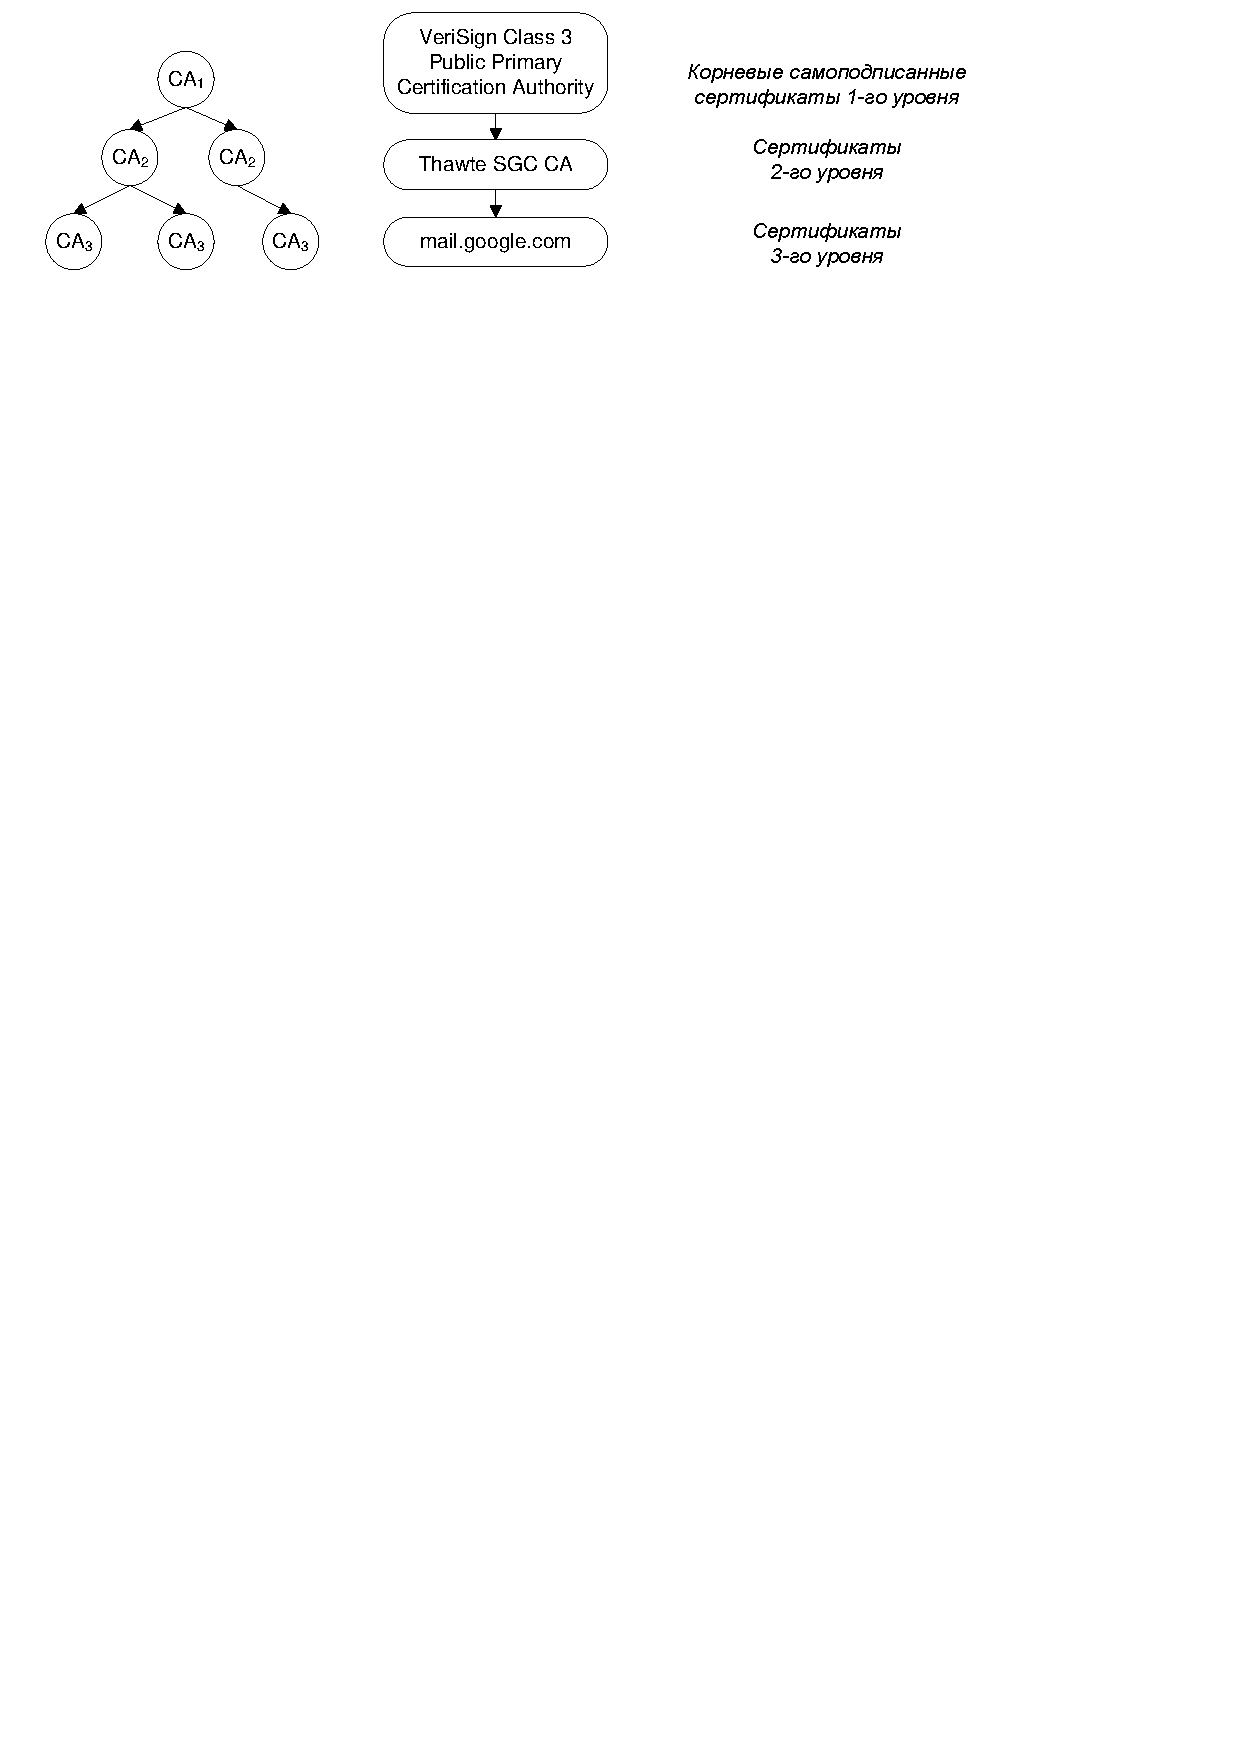
\includegraphics[width=0.8\textwidth]{pic/X509-hierarchy}
	\caption{Иерархия сертификатов\label{fig:x509-hierarchy}}
\end{figure}

На рис.~\ref{fig:x509-hierarchy} приведены примеры иерархии сертификатов и путь подписания сертификата X.509\index{сертификат!X509} интернет-сервиса Gmail (Google Mail).

Система распределения, хранения и управления сертификатами открытых ключей называется \emph{инфраструктурой открытых ключей}\index{инфраструктура открытых ключей} (\langen{public key infrastructure, PKI}). PKI применяется для аутентификации в системах SSL/TLS\index{протокол!SSL/TLS}, IPsec\index{протокол!IPsec}, PGP и~т.\,д. Помимо процедур выдачи и распределения открытых ключей, PKI также определяет процедуру отзыва скомпрометированных или устаревших сертификатов.


\subsection{Структура сертификата X.509}
\selectlanguage{russian}

Ниже приведён пример сертификата X.509\index{сертификат!X509}, использовавшегося интернет-сервисом mail.google.com для предоставления защищённого SSL-соединения в 2009 г. Сертификат напечатан командой \texttt{openssl x509 -in file.crt -noout -text}:

{\small \begin{verbatim}
Certificate:
Data:
  Version: 3 (0x2)
  Serial Number:
    6e:df:0d:94:99:fd:45:33:dd:12:97:fc:42:a9:3b:e1
  Signature Algorithm: sha1WithRSAEncryption
  Issuer: C=ZA, O=Thawte Consulting (Pty) Ltd.,
    CN=Thawte SGC CA
  Validity
    Not Before: Mar 25 16:49:29 2009 GMT
    Not After : Mar 25 16:49:29 2010 GMT
  Subject: C=US, ST=California, L=Mountain View, O=Google Inc,
    CN=mail.google.com
  Subject Public Key Info:
    Public Key Algorithm: rsaEncryption
    RSA Public Key: (1024 bit)
      Modulus (1024 bit):
        00:c5:d6:f8:92:fc:ca:f5:61:4b:06:41:49:e8:0a:
        2c:95:81:a2:18:ef:41:ec:35:bd:7a:58:12:5a:e7:
        6f:9e:a5:4d:dc:89:3a:bb:eb:02:9f:6b:73:61:6b:
        f0:ff:d8:68:79:1f:ba:7a:f9:c4:ae:bf:37:06:ba:
        3e:ea:ee:d2:74:35:b4:dd:cf:b1:57:c0:5f:35:1d:
        66:aa:87:fe:e0:de:07:2d:66:d7:73:af:fb:d3:6a:
        b7:8b:ef:09:0e:0c:c8:61:a9:03:ac:90:dd:98:b5:
        1c:9c:41:56:6c:01:7f:0b:ee:c3:bf:f3:91:05:1f:
        fb:a0:f5:cc:68:50:ad:2a:59
      Exponent: 65537 (0x10001)
  X509v3 extensions:
    X509v3 Extended Key Usage: TLS Web Server
      Authentication, TLS Web Client Authentication,
      Netscape Server Gated Crypto
    X509v3 CRL Distribution Points:
    URI:http://crl.thawte.com/ThawteSGCCA.crl
    Authority Information Access:
    OCSP - URI:http://ocsp.thawte.com
    CA Issuers - URI:http://www.thawte.com/repository/
        Thawte_SGC_CA.crt
    X509v3 Basic Constraints: critical
    CA:FALSE
Signature Algorithm: sha1WithRSAEncryption
  62:f1:f3:05:0e:bc:10:5e:49:7c:7a:ed:f8:7e:24:d2:f4:a9:
  86:bb:3b:83:7b:d1:9b:91:eb:ca:d9:8b:06:59:92:f6:bd:2b:
  49:b7:d6:d3:cb:2e:42:7a:99:d6:06:c7:b1:d4:63:52:52:7f:
  ac:39:e6:a8:b6:72:6d:e5:bf:70:21:2a:52:cb:a0:76:34:a5:
  e3:32:01:1b:d1:86:8e:78:eb:5e:3c:93:cf:03:07:22:76:78:
  6f:20:74:94:fe:aa:0e:d9:d5:3b:21:10:a7:65:71:f9:02:09:
  cd:ae:88:43:85:c8:82:58:70:30:ee:15:f3:3d:76:1e:2e:45:
  a6:bc
\end{verbatim}}

Как видно, сертификат действителен с 26.03.2009 до 25.03.2010, открытый ключ представляет собой ключ RSA\index{криптосистема!RSA} с длиной модуля $n = 1024$ бита и экспонентой $e = 65537$ и принадлежит компании Google Inc. Открытый ключ предназначен для взаимной аутентификации веб-сервера mail.google.com и веб-клиента в протоколе SSL/TLS. Сертификат подписан ключом удостоверяющего центра Thawte SGC CA, подпись вычислена с помощью криптографического хеша SHA-1\index{хеш-функция!SHA-1} и алгоритма RSA\index{электронная подпись!RSA}. В свою очередь, сертификат с открытым ключом Thawte SGC CA для проверки значения ЭП данного сертификата расположен по адресу: \url{http://www.thawte.com/repository/Thawte\_SGC\_CA.crt}.

Электронная подпись вычисляется от всех полей сертификата, кроме самого значения подписи.

